\documentclass{article}
\usepackage{tikz}
\usepackage{amsmath}
\usepackage[a4paper]{geometry}
\usepackage{fancyhdr}
\pagestyle{fancy}
\lhead{Starke Kernkraft beim Alpha-Zerfall}
\rhead{Januar 2026}
\begin{document}
\section{Starke Kernkraft beim Alpha-Zerfall}
Die starke Kernkraft wirkt mit einer Reichweite von $1,5\,\text{fm}$ zwischen Nukleonen im Kern anziehend um die Protonen zusammen zu halten.
 
\subsection{Das Problem} 
Es wäre davon auszugehen dass das $\alpha$-Teilchen seine Energie aus der Coulombkraft zwischen dem $\alpha$-Teilchen und dem Element, hier als Beispiel Am-$241$, gewinnt, welche anfängt, sobals es der starken Kernkraft entkommen ist.
\[
 E = \int F_c\,\text{d}s 
\]
Die Distanz zwischen den Zentern der beiden Ladungsträgern ab welcher das Teilchen der starken Kernkraft entkommen sind die obigen $1,5\,\text{fm}$ plus die beiden Radien, sowohl des Elements als auch des $\alpha$-Teilchens.
\[
 r_A = 1,5\,\text{fm} + r_\alpha + r_E
\]
Der Coulombkraft nach folgt nun 
\[ 
 E_{kin} = \int_{r_A}^\infty 
 \frac{1}{4 \pi \epsilon_0} \cdot \frac{Q_\alpha \cdot Q_E}{r^2}
 \,\text{d}r
\]
$Q_\alpha$ und $Q_E$ sind jeweils die $2e$ und die Anzahl der Elektronen des Elements.
 
Im fall von Am-$241$ sind das $93e$. Hier folgt dann $E_{kin} \approx 21,8\,\text{MeV}$. Das Spektrum der gemessenen Energien endet aber bei $5,55\,\text{MeV}$.
 
\subsection{Der Tunneleffekt} 
Die Coulombkraft dürfte erst ab $\approx 37\,\text{fm}$ anfangen zu wirken damit die Energien übereinstimmen würden. Dies wird durch den \emph{Tunneleffekt} ermöglicht; ein Quanteneffekt der der klassischen Physik widerspricht.
 
Hier liegen, analog zum Potentialtopf der Farbstoffmoleküle, die Protonen und Neutronen des Kerns als Materiewellen (de Broglie-Wellen) vor.
 
Emittiert ein Kern ein $\alpha$-Teilchen, so gehen die anderen Protonen und Neutronen in energetisch niedrigere Zustände über. Diese spezifischen Vorgänge führen zu spezifischen $E_{kin}$ der $\alpha$-Teilchen und $\gamma$-Quanten. 
\begin{center}
 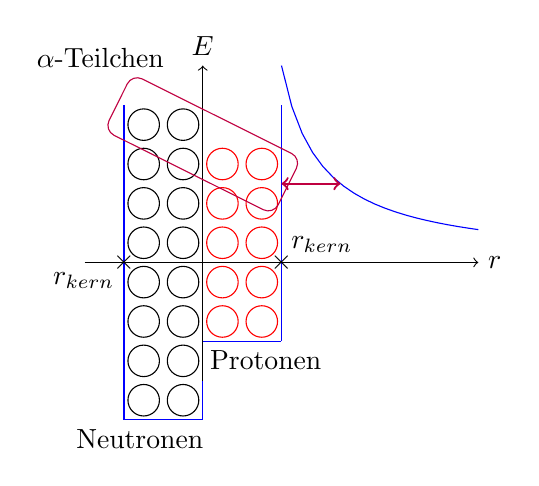
\begin{tikzpicture}
  \draw[->] (-1.5, 0) -- (3.5,0) node[right]{$r$};
  \draw[->] (0, -2) -- (0,2.5) node[above]{$E$};
 
  \draw[blue] (-1, 2) -- (-1,-2);  
  \draw[blue] (-1, -2) -- (0,-2);
  \draw[blue] (0, -2) -- (0,-1.5); 
  \draw[blue] (0, -1) -- (1,-1);
  \draw[blue] (1, -1) -- (1,2); 
  
  \node at (-1, 0) {$\times$}; 
  \node[below left] at (-1, 0) {$r_{kern}$};  
  \node at (1, 0) {$\times$};
  \node[above right] at (1, 0) {$r_{kern}$};
 
  \node at (-0.8, -2) [below]{Neutronen}; 
  \node at (0.8, -1) [below]{Protonen};
 
  \foreach \y in {-2,...,5} { 
   \foreach \x in {-2, -1} { 
    \draw ({\x/2+0.25}, {\y/2-0.75}) circle (0.2);
   };
  } 
  \foreach \y in {0,...,4} { 
   \foreach \x in {0, 1} { 
    \draw[red] ({\x/2+0.25}, {\y/2-0.75}) circle (0.2);
   };
  }
  
  \draw[purple, rounded corners, rotate around={-26.5:(0,1.5)}] 
    (-1.2, 1.1) rectangle (1.2, 1.9);
  \node at (-1.3, 2.6){$\alpha$-Teilchen};
  
  \draw[blue, domain=1:3.5, samples=20] plot (\x, {1/((\x-0.5))/2*2.5});
  \draw[<->, purple, thick] (1, 1) -- (1.75,1); 
 \end{tikzpicture} 
\end{center} 
Der Coulombwall ist nicht unendlich breit; die Aufenthaltswahrscheinlichkeit ist nicht mehr null.
\[
 E = \frac{1}{4\pi\epsilon_0} \cdot \frac{Q_1Q_2}{r} 
\] 
\end{document}